\cotefile{157-1}
\scanpage{150}\mspage{8}
L'\unsure{augmentation} canonique
\[
 L\alpha_!(k_{C'})\longrightarrow k_C
\]
redonne, en prenant les $R\mathrm{Hom}$ dans $F$
\[
 \unsure{\mathbb R|\mathrm R}\Gamma(C,F)\longrightarrow
 R\mathrm{Hom}(L\alpha_!(k_{C'}),F)
 \xleftarrow{\sim}\mathbb R\Gamma(C',\alpha^*F)
\]
l'hom canonique de ``contravariance'' de la coh.

Si par contre on travaille sur le dérivateur \unsure{non} additif $\mathrm{HOT}$, avec $F$ un
``type d'homotopie relatif'' sur $C$'', \deleted{qu'}on doit avoir
\diagram{\fbox{\begin{tikzcd}[ampersand replacement=\&,column sep=0pt,row sep=small]
 \mathbb R\Gamma_{\mathrm{HOT}}(C',\alpha^*F)\arrow[r,"\sim"] \&
 \inserted{\mathbb R\Gamma(C,}\deleted{\unsure{R}}\mathrm{Hom}\,(\alpha_!( \&
 e_{C'} \& ),F))\\
 {} \& \substack{\text{Hom interne}\\\text{de la cat. des}\\\text{types d'hom.}\\\text{relatifs sur }C}\arrow[u] \&
 \substack{\text{objet}\\\text{final de}\\\mathrm{HOT}(C')\\\text{type d'h. rel.}\\\text{final sur }C'}\arrow[u,<->] \& {}
\end{tikzcd}}}
En fait, ces formules sont \unsure{quasi-tautologiques}, si on admet l'existence des foncteurs $\alpha_!$ \unsure{comme|commes} \unsure{adjoints} à \uline{gauche} des $\alpha^*$. \deleted{\unsure{Dans}} le cas abélien, \inserted{\unsure{disons|lisons},}
\diagram{\begin{tikzcd}[ampersand replacement=\&,column sep=small,row sep=small]
 C'\arrow[rr,"\alpha",dash]\arrow[dr,"f'"'] \& \& C\arrow[dl,"f",dash]\\
 \& e \&
\end{tikzcd}}
\deleted{\[
 \mathbb R\Gamma(C',\alpha^*(F))\in\mathrm{\unsure{Dér|Der}}(k\text{-}\mathrm{Ab})=D
\]}
\deleted{représente le foncteur \unsure{cov.|suiv.} sur $D$}
\deleted{\[
 \begin{aligned}
 G&\longmapsto\mathrm{Hom}(G,
 \underbrace{\mathbb R\Gamma(C',\alpha^*F)}_{
 \substack{\|\,\text{déf}\\ f'_{*}(\alpha^*(F))}})
 \simeq\mathrm{Hom}_{C'}(G_{C'},\alpha^*(F))\\
 &\hspace{13em}\substack{\|\,\text{adj.}}\\[-2pt]
 &\hspace{9em}\mathrm{Hom}_{C}(\underbrace{\alpha_!(G_{C'})}_{
 \substack{\|\\\alpha_!{\underbrace{\alpha^*(G_C)}_{\unsure{?}}}}},F)
 \end{aligned}
\]}
% archive sheet number: 150
\scanpage{151}
\mspage{9}
\deleted{tandis que le deuxième \unsure{mb|est} représente (compte tenu que
$\unsure{\mathbb R|\mathrm R}\mathrm{Hom}=\mathbb R\Gamma(C,\mathbb R\underline{\mathrm{Hom}})$}
\deleted{\[
 \mathrm{Hom}_{C}(G_C,R\underline{\mathrm{Hom}}(L\alpha_!(k_{C'}),F)
 \simeq\mathrm{Hom}_{C}(L\alpha_!(k_{C'}
\]}
L'isomorphie des $H^0$ des deux \unsure{mbs|mbres} est la formule d'adjonction
\[
 \mathrm{Hom}_{C'}(k_{C'},\alpha^*F)\simeq\mathrm{Hom}_C(\alpha_!(k_{C'}),F)
\]
d'où l'isomorphie pour les $H^i$ des deux mbs, par décalage.
De $=$ dans le cas de $\mathrm{HOT}$, l'isomorphie can. des $\pi_0$ des deux mbs est la formule d'adjonction.
Pour avoir l'isomorphisme plus fin dans $\mathbb D(e)$, la cat. \unsure{fondamentale} du dérivateur envisagé) en \unsure{termes|terme} de Hom \unsure{internes|interne},
on doit \deleted{\unsure{utili}} admettre l'existence d'objets unité (\inserted{les} $k_X$ dans un cas, \inserted{les} $e_X$ dans l'autre), compatible avec \unsure{image inverse|images inverses}, de telle façon
\[
 \mathrm{Hom\,int}(\unsure{\varepsilon|\mathcal E}_X,\underset{\substack{\rotatebox{-90}{$\in$}\\\mathbb D_X}}{F})\simeq F .
\]
On aura
\[
 \Gamma(C',\alpha^*F)\overset{\text{déf}}{\simeq} f'_*(\alpha^*(F))\simeq
 f_*\deleted{(\unsure{\mathrm{Hom\,int}}(\varepsilon_{C'},\unsure{\alpha^*}(F)))}\inserted{(\alpha_*\alpha^*F)} ,
\]
Et la question est donc de \unsure{donner|dégager} une interprétation de $\alpha_*\alpha^*F$ comme
\[
 \alpha_*\alpha^*F\simeq\mathrm{Hom\,int}(\alpha_!(\varepsilon_{C'}),F)
 \qquad\text{dans }\mathbb D(C)
\]
Pour ceci, on va écrire
\[
 \alpha^*F,\simeq\mathrm{Hom\,int}(\varepsilon_{C'},F),
\]
et la formule doit résulter d'une ``formule d'adjonction interne''
% archive sheet number: 151
\scanpage{152}
\mspage{10}
\margin{?}
\[
 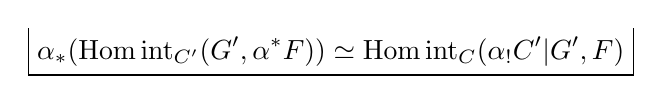
\begin{tikzpicture}[baseline=(eq.base)]
 \node[inner sep=3pt] (eq) {$\displaystyle\alpha_*(\mathrm{Hom\,int}_{C'}(G',\alpha^*F))\simeq
 \mathrm{Hom\,int}_{C}(\alpha_!\unsure{C'|G'},F)$};
 \draw (eq.north west)--(eq.south west)--(eq.south east)--(eq.north east);
 \end{tikzpicture}
\]
(\uline{Formule d'adjonction} ``\uline{interne}'', pour $\alpha_!$ et $\alpha^*$,
valable en principe pour \uline{\unsure{tte|tt}} $\alpha:C'\longrightarrow C$ dans $\mathrm{Diag}$. \unsure{tout} $G'$ dans $\mathbb D(C')$ et tout $F$ dans $\mathbb D(C)$.

Comment prouver cette formule ? En prenant l'opération produit $\otimes$, associée à l'\unsure{op|hop} Hom int, on est ramené \inserted{(en prenant les foncteurs contr. associés)} à une formule
\[
 G\otimes\alpha_!G'\xrightarrow{\sim}\alpha_!(\alpha^*\unsure{C|G}\otimes C')\unsure{,|/}
\]
\deleted{Si $G$ est de la forme $f^*G_0$ (\unsure{coeff|coeff.} \uline{constant} sur $C$)}

On trouve par adjonction un hom can $\unsure{-|\longrightarrow}$, il faut voir s'il est tjrs iso.
% archive sheet number: 152
\scanpage{153}
\mspage{11}
2. \inserted{\unsure{les}}\uline{Catégories loc. filtrantes} \uline{sont} \uline{les catégories loc. \deleted{\unsure{filtrantes}} \inserted{tot. \unsure{0-connexes}}} ?

Soit $\mathscr T$ un topos. On dit que $\mathscr T$ est \uline{irréductible} \deleted{\unsure{s'il est dans}} si l'ens. ordonné \inserted{$\mathrm{Ouv}(\mathscr T)$,} des sous-\deleted{\unsure{b}}objets \deleted{\unsure{ouverts}} \inserted{de $e_{\mathscr T}$} \deleted{\unsure{de $\mathscr T$}} a la propriété suivante :
a) $\mathrm{Ouv}(\mathscr T)$ n'est pas réduit à un élément, i.e. $\varnothing_{\mathscr T}\to e_{\mathscr T}$ n'est pas un isomorphisme ($\mathscr T$ n'est pas identique \deleted{\unsure{au}} au sous-topos vide).
b) Si $U',U''$ sont deux objets ``non vides'' i.e. non initiaux de $\mathrm{Ouv}(\mathscr T)$, leur \unsure{produit,} intersection est ``non vide''.
Il revient au $=$ de dire que si $\mathscr T',\mathscr T''$ sont deux sous-topos fermés distincts de $\mathscr T$, alors \deleted{$\mathscr T'\vee\mathscr T''$} leur \unsure{sup} $\mathscr T'\vee\mathscr T''$ est distinct de $\mathscr T$, \inserted{ou encore que tt ouvert de $\mathscr T$ est connexe.}
% slanted
\margin{\uline{NB} Irréductible n'implique \unsure{pas} loc irréductible, pas plus que connexe n'implique loc. connexe etc}

On dit que $\mathscr T$ est \uline{loc. irréductible} si \deleted{tout objet \unsure{0-conn}}
a) $\mathscr T$ est loc connexe, \deleted{et si tout objet} (i.e. chaque faisceau sur $\mathscr T$ est somme de faisceaux 0-connexes),
et si \inserted{b)} pour tt faisceau 0-connexe \inserted{$U$} sur $\mathscr T$, le topos induit $\mathscr T_{/U}$ est irréductible \unsure{,|.} [i.e. l'ens \deleted{\unsure{ord}} ordonné $\mathrm{Ouv}(U)$ des sous-objets de $U$\unsure{,} a la propriété b) ci-dessus (a) signifiant \unsure{simpl\textsuperscript{t}} que \deleted{$U\unsure{\ne}\varnothing_{\mathscr T}$} $U\unsure{\not\simeq|\ne}\varnothing_{\mathscr T}$\unsure{\}}, i.e. que $U$ n'est pas objet initial dans $\mathscr T^{\wedge}$\unsure{\}}, ou plus \unsure{simple|simplet},] : \deleted{un sous-objet} tout sous-faisceau d'un faisceau \deleted{connexe} \unsure{est} connexe.
% margin note written sideways
\margin{$\mathscr T$ est loc irréductible ssi il a une famille génératrice $(U_\alpha)$, avec les $U_\alpha$ ``irréductibles'' (\unsure{donc} $0$-connexes -- \unsure{donc} $\mathscr T$ est loc. \deleted{\unsure{con}} connexe \unsure{?})}

Quand $\mathscr T$ est de la forme \deleted{\unsure{Top}} $\mathrm{Top}(T)$, où $T$ est un espace topologique, dire $\mathscr T$ irréductible signifie que $T$ est irréductible (car alors $\mathrm{Ouv}(\mathscr T)\simeq\mathrm{Ouv}(T)$\deleted{\unsure{\})}})\unsure{;} \deleted{et le fait \unsure{que}} \deleted{\unsure{connexe tt}} dire \inserted{\unsure{triv.}} que $T$ est loc connexe,
\deleted{et $\mathscr T$ est loc. connexe} (\deleted{\unsure{tout}} tout ouvert est somme \inserted{disj.} d'ouverts connexes), donc $\mathrm{Top}(T)$ est loc connexe. De plus, cel\unsure{a} implique aussi que $\mathrm{Top}(T)$ est loc. irréductible*. (\uline{NB} les objets 0-connexes
% slanted
\margin{expliciter la démonstration.}
% archive sheet number: 153
\scanpage{154}
\mspage{12}
% archive sheet number: 154
de $\mathrm{Top}(T)^\wedge$, i.e. les faisceaux d'ens. \inserted{$F$} 0-connexes sur $T$, sont ceux dont la ``fibre générique'' a exactement un point \unsure{...|ou.})
\inserted{Ainsi $\mathscr T=\mathrm{Top}(T)$ est loc. irr. ssi $T$ loc. connexe, et les comp. connexes de $T$ sont \unsure{irr.} irréductibles, i.e. ssi $T=\coprod_i T_i$, les $T_i$ irréductibles.}

Si $\mathscr T$ est de la forme $\mathrm{Top}(X)$, $X$ une catégorie, \unsure{où|on} sait que $\mathscr T$ est loc. connexe (et \unsure{$=^t$} localement $\infty$-connexe).
On voit \deleted{donc} que $\mathscr T$ est irréductible ssi $\mathrm{Esp}(X)$ (l'espace topologique associé, dont l'ens. sous-jacent est $\mathrm{Ob}\,X$) est irréductible\inserted{*}.
% slanted
\margin{* Car les ouverts de $\mathrm{Top}(X)$, ceux de $\mathrm{Esp}(X)$ et ceux de $X$, \unsure{s'identifient}. (\deleted{\unsure{NB}} Cela signifie (ssi) que pour $x,y$ dans $X$, $\exists z$ \unsure{avec}
\diagram{\begin{tikzcd}[ampersand replacement=\&,row sep=0pt,column sep=small]
 \& x\\ z\arrow[ur]\arrow[dr] \& {}\\ \& y
\end{tikzcd}}
\unsure{;} i.e. $\mathrm{Ord}(X)$ est filtrant à \unsure{g.}}
On \deleted{\unsure{définira}} dit alors que $X$ est irréductible. \deleted{\unsure{ssi}} Comme les composantes connexes de $X$ et celles de $\mathrm{Esp}(X)$ \inserted{ou $\mathrm{Top}(X)=\mathscr T$} se correspondent, on voit donc que \deleted{\unsure{les}} les conditions suivantes sont équivalentes :
\textcircled{a} \inserted{le topos} $\mathrm{Top}(X)$ est loc. irr. \quad b) $\mathrm{Esp}(X)$ est loc. irréductible \quad c) les composantes connexes de \deleted{\unsure{objets}} $X$ sont irréductibles\unsure{;} \inserted{\textcircled{d} les $X_{/x}$ irréductibles,}
On dit alors que $X$ est \deleted{loc.} irréductible.
% slanted
\margin{Faux, on a
\diagram{\begin{tikzcd}[ampersand replacement=\&,row sep=small]
 (a\Longleftrightarrow d)\arrow[d,Rightarrow]\\
 (b\Longleftrightarrow c)
\end{tikzcd}}}
% slanted
\margin{$X$ irréductible n'implique \uline{pas} que $X_{/x}$ le soient, exemple
\diagram{\begin{tikzcd}[ampersand replacement=\&,column sep=small]
 X={} \& 0\arrow[r,bend left,"\alpha"]\arrow[r,bend right,"\beta"'] \& 1 \& (\alpha\ne\beta),
\end{tikzcd}}
on a
\diagram{\begin{tikzcd}[ampersand replacement=\&,row sep=0pt,column sep=small]
 \& 0'\arrow[dr]\\ X_{/1}=\deleted{\unsure{0}} \& \& 1\\
 \&0''\arrow[ur]
\end{tikzcd}}
\unsure{qui} n'est \uline{pas} irréductible, \deleted{\unsure{et n'est pas localement irréductible}} ni \unsure{localt irrd.|localt itou} puisqu'il est connexe. Pourtant il est étale sur $X$.}
\deleted{Il \unsure{reviendra}} Cela implique donc que pour \deleted{tout objet \unsure{0-connexe}} $X'$ étale sur $X$, $X'$ 0-connexe, $X'$ est irréductible.
\inserted{\uline{Dire conditions équivalentes} \textcircled{a} $\mathrm{Top}(X)$ est loc. irr.
\textcircled{b} les $X_{/x}$ irréductibles \textcircled{c} \deleted{tout} objet 0-connexe de $X^\wedge$ est irréductible (i.e. \unsure{tt} \unsure{s.-obj.} $\ne\varnothing$ \unsure{etc}),
\deleted{\textcircled{d} les \unsure{commas} de $X$ \unsure{sont irréductibles}} \textcircled{e} conditions de \deleted{\unsure{SGA}} $\mathrm{SGA}\,4$ \unsure{I 2|I § 2}}
Si \deleted{$X$ est \unsure{Cat.} \unsure{vide}} \inserted{$X\ne\varnothing$ et} $X$ irréductible signifie \deleted{\unsure{ssi}} que $\forall\,x,y\in\mathrm{Ob}\,X$, existe $s$ \deleted{\unsure{et deux}}
\diagram{\begin{tikzcd}[ampersand replacement=\&,row sep=0pt,column sep=small]
 \& x\\ s\arrow[ur]\arrow[dr] \& {}\\ \& y
\end{tikzcd}}
. (Cela signifie que $X$ est \uline{fbt. filtrante}* à gauche, faiblement cofiltrante).
$X$ loc. \deleted{\unsure{filtr}} irréd signifie que pour $x,y$ \deleted{\unsure{qq}} \uline{appartenant à une \unsure{même} comp. connexe}, existe $s$ avec
\diagram{\begin{tikzcd}[ampersand replacement=\&,row sep=0pt,column sep=small]
 \& x\\ s\arrow[ur]\arrow[dr] \& {}\\ \& y,
\end{tikzcd}}
% slanted
\margin{* Il vaut mieux l'appeler \uline{pseudo-filtrante}, et réserver ``loc. \unsure{filt.}'' (= fbt. filtrante $\unsure{+}$ connexe).}
\scanpage{155}
\mspage{13}
i.e. $X_{/[x]}\cap X_{/[y]}\ne\varnothing$ [où $[x]$ est \deleted{\unsure{l'id$(x)$}} \inserted{$x$} considéré comme \deleted{objet} \inserted{élément} de l'ens ordonné $\mathrm{Ob}\,X$].
Il \unsure{revient aussi|revient encore} au $=$ de dire que les catégories induites $\deleted{\unsure{I}}X_{/x}$ sont \unsure{irréductible|irréductibles}.
% slanted
\margin{faux cf \unsure{aussi le|aussi} \unsure{contre-exemple} \unsure{précédent|précédente}}

\deleted{\unsure{Comme}} \uline{Exemple} Une catégorie \uline{ayant un objet initial}, ou seulement un ``plus petit objet'', est irréductible.
\deleted{\unsure{Donc aussi|D'une manière} toute catégorie dont tte composante connexe admet un plus petit objet, est loc. irréductible.}
Inversement, si l'ens \uline{ordonné} $\mathrm{Ord}(X)$ associé à $X$ [quotient de $\mathrm{Ob}\,X$ par la relation d'équivalence associée à son préordre] est fini, p. ex. $X$ fini, \deleted{donc} ou seulement loc fini, p. ex. $X$ loc. fini (i.e. les catégories $X_{/x}$ finies), alors si $X$ est irréductible, $\mathrm{Ob}\,X$ a un plus petit élément i.e. $X$ a un plus petit objet.
C'est vrai plus gén. encore, si $\mathrm{Ord}(X)$ est artinien, i.e. \deleted{toute} toute suite décroissante dans $\mathrm{ord}(X)$ est stationnaire. //
Mais la condition intéressante est la condition \unsure{toposique} de \uline{locale} irréductibilité, qui équivaut à $I$ pseudo-filtrante \inserted{\unsure{à g.}}, i.e. les comp. connexes de $I$ \deleted{pseudo-}filtrantes, i.e. les conditions $\mathrm{PS}1$, $\mathrm{PS}2$
\uline{PS1} Tout diagramme
\diagram{\begin{tikzcd}[ampersand replacement=\&,row sep=0pt,column sep=small]
 x\arrow[dr] \& {}\\ {} \& s\\ y\arrow[ur] \& {}
\end{tikzcd}}
se complète en
\diagram{\begin{tikzcd}[ampersand replacement=\&,row sep=0pt,column sep=small]
 \& x\arrow[dr] \& {}\\ z\arrow[ur]\arrow[dr] \& {} \& s\\ \& y\arrow[ur] \& {}
\end{tikzcd}}
\uline{commutatif}

\uline{PS2} Pour \unsure{tte|tt} double flèche $x\rightrightarrows y$, existe un égalisateur
\diagram{\begin{tikzcd}[ampersand replacement=\&,column sep=small]
 z\arrow[r] \& x\arrow[r,shift left]\arrow[r,shift right] \& y
\end{tikzcd}}
\deleted{\unsure{est} \unsure{commutatif} \unsure{ou} $\unsure{z\to x}$ \unsure{(égalise)} \illegible{1}}
% archive sheet number: 155
\scanpage{156}
\mspage{14}
\deleted{Proposition}

En résumé, on a la

\uline{Proposition} 2.1. Soit $X$ \unsure{une|un} objet de $\mathrm{Cat}$. Conditions équivalentes :
a) Le topos associé $\mathrm{Top}(\unsure{x|X})$ est loc. irréductible, i.e. \deleted{pour} (\unsure{étant} loc. connexe) pour \deleted{tout} objet \deleted{de} $F$ de \deleted{\unsure{Top}} $X^\wedge$ et tout sous-objet $F'$ de $F$, si $F$ est connexe $F'$ l'est.

a') Pour tt $X'$ étale sur $X$, si $X'$ est connexe, \deleted{\unsure{tout|tt}} ouvert de $X'$ est connexe.

a'') Tout ouvert d'une catégorie localisée $X_{/a}$ \inserted{($a\in\mathrm{Ob}\,X$)} est connexe, \inserted{(i.e. $X_{/a}$ est une cat. irréductible, i.e. le topos $\mathrm{Top}(X_{/a})$ l'est).}

\deleted{a''') Pour tt $a\in\mathrm{Ob}\,X$, \unsure{$E= (\mathrm{Ob}\,X)$} $\mathrm{Esp}(X_{/a})$ est irréductible.}
\inserted{b) \deleted{est \unsure{fl}} Pour \deleted{tout} objet $a$ de $X$, $\mathrm{Esp}(X_{/a})$ est un espace topologique irréductible.}

\unsure{b)} Les catégories $X_{/a}$ sont \deleted{\unsure{pseudo-}}\inserted{faiblement} filtrantes \deleted{i.e.} à gauche (ou \unsure{fbt} cofiltrantes), i.e. pour deux objets $\xi,\eta$ d'une telle catégorie, existe \inserted{un objet} $\zeta$ et deux flèches
\diagram{\begin{tikzcd}[ampersand replacement=\&,row sep=0pt,column sep=small]
 \& \xi\\ \zeta\arrow[ur]\arrow[dr] \& {}\\ \& \eta
\end{tikzcd}}
(\unsure{donc|i.e.} l'ens ordonné \inserted{$\mathrm{Ord}(X_{/a})$} associé à $X_{/a}$ est filtrant à gauche)

\unsure{b'|c'}) Pour \deleted{deux flèches} tout diagr. en traits pleins de $X$
\diagram{\begin{tikzcd}[ampersand replacement=\&,row sep=small,column sep=small]
 \& x\arrow[dr] \& {}\\ z\arrow[ur,dotted]\arrow[dr,dotted] \& {} \& a,\\
 \& y\arrow[ur] \& {}
\end{tikzcd}}
on peut le compléter en un carré \uline{commutatif} comme indiqué (Condition PS1 des cat. loc. filtrantes)
\deleted{\unsure{c)} \unsure{Toute} Toute composante connexe de $X$}
Ces conditions impliquent que tte composante connexe $X_\alpha$ de $X$ est irréductible, ou ce qui revient au $=$, que $\mathrm{Esp}(X_\alpha)$ est irréductible,
% archive sheet number: 156
\scanpage{157}
\mspage{15}
mais ne sont pas impliquées par celles-ci.

Contr'exemple, la catégorie 0-connexe
\diagram{\begin{tikzcd}[ampersand replacement=\&,column sep=small]
 0\arrow[r,bend left,"\alpha"]\arrow[r,bend right,"\beta"'] \& 1
\end{tikzcd}}
, avec $\alpha\ne\beta$. \unsure{On a|Car.} \deleted{\unsure{$D=$}} $X_{/1}\simeq$
\diagram{\begin{tikzcd}[ampersand replacement=\&,row sep=0pt,column sep=small]
 \& \unsure{0|0'}\arrow[dr] \& {}\\
 \deleted{\unsure{0}}\arrow[ur,dash,"\deleted{\unsure{\alpha}}"]\arrow[dr,dash,"\deleted{\unsure{\beta}}"'] \& {} \& 1\\
 \&0'\arrow[ur] \& {}
\end{tikzcd}}
, qui n'est pas irréductible, puisque $\unsure{D|\Phi}\smallsetminus\{1\}$ \inserted{$\simeq\unsure{2|e}$} est un ouvert \unsure{disconnexe|déconnexe}.

J'aimerais une condition ``toposique'' sur $X$, équivalente à \deleted{\unsure{$I$}} $X$ ``pseudofiltrante à gauche'' i.e. les composantes connexes filtrantes ; i.e. $\mathrm{PS}\underline{1}^{\mathrm{opp}}$ (condition \unsure{c'|b'}\unsure{)} ci-dessus) $+$ $\mathrm{PS}2^{\mathrm{opp}}$ (condition de la double flèche), et qui de plus implique que tout objet \inserted{0-}connexe de $X^\wedge$ (i.e. tt objet $X'$ de $\mathrm{Cat}$ étale sur $X$ et 0-connexe) soit $W_\infty$-asphérique. Et je songe à la notion des ``\unsure{totally asphericats|totales asphéricités}'' de PS (\unsure{Pursuing Stacks}).

\uline{Définition} \unsure{a)} 2.2. Soit $X$ une catégorie. \deleted{\unsure{a}}
% slanted
\margin{Cf tableau récapitulatif pages 97, 98 et surtout 99}
On dit que $X$ est \uline{faiblement filtrante}* \deleted{(ou \unsure{fbt.} filtrante} \uline{à gauche} \inserted{ou \uline{irréductible}}, \deleted{ou \unsure{quand}} si $X\ne\varnothing$, et si pour $a,b\in\mathrm{Ob}\,X$ $\exists c$ et des flèches
\diagram{\begin{tikzcd}[ampersand replacement=\&,row sep=0pt,column sep=tiny]
 \& a\\ c\arrow[ur]\arrow[dr] \& {}\\ \& b
\end{tikzcd}}
, i.e. $\deleted{\unsure{X}} X_{/(a)}\cap\deleted{\unsure{X}}X_{/[b]}\ne\varnothing$.
% slanted
\margin{dire plutôt \uline{pseudo-filtrante} \unsure{(puisque)} \unsure{réserver|c'est une} \unsure{appellation} loc. fbt filtrante'' condition PS $\underline{1}'_{\mathrm g}$}
(\uline{NB} $X$ est ps. filtr. \inserted{à g.} ssi $\mathrm{Ord}(X)$ \inserted{(i.e. est filtr. à g)} l'est.)
\uline{ReNB} $X$ fbt filtrante $\Longrightarrow X$ 0-connexe

b) On dit que $X$ est \uline{loc. faiblement filtrante} \deleted{\unsure{si}} ou
\inserted{\uline{ou plus simpl. $\longrightarrow$ loc. filtrante à gauche}} \deleted{les catégories} \uline{à gauche}, \deleted{\unsure{ou ps.}} si les catégories $X_{/x}$ ($x\in\mathrm{Ob}\,X$) sont fbt filtrantes à gauche, i.e. si $X$ satisfait la condition : $\forall$ diagramme
\diagram{\begin{tikzcd}[ampersand replacement=\&,row sep=0pt,column sep=small]
 a\arrow[dr] \& {}\\{} \&x,\\ b\arrow[ur] \&{}
\end{tikzcd}}
$\exists c$ de $X$ et des flèches de $c$ dans $a,b$ rendant \uuline{commutatif} le carré
% slanted
\margin{condition PS $1_{\mathrm g}$}
\diagram{\begin{tikzcd}[ampersand replacement=\&,row sep=0pt,column sep=small]
 \& a\arrow[dr] \& {}\\ c\arrow[ur,dotted]\arrow[dr,dotted] \&{} \&x\\ \& b\arrow[ur] \&{}
\end{tikzcd}}
[\uline{NB} Cette condition \deleted{n'est pas} implique que $\mathrm{Ord}\,X$ soit loc fbt filtrante, mais n'équivaut pas à cette dernière. Exemple $X={}$%
\diagram{\begin{tikzcd}[ampersand replacement=\&,column sep=small]
 0\arrow[r,bend left,"\alpha"]\arrow[r,bend right,"\beta"'] \&1
\end{tikzcd}}
, $X_{/1}={}$%
\diagram{\begin{tikzcd}[ampersand replacement=\&,row sep=0pt,column sep=small]
 0'\arrow[dr] \&{}\\ {} \&1\\ 0''\arrow[ur] \&{}
\end{tikzcd}}
n'est pas \unsure{faib.} filtr. à g.]
% archive sheet number: 157
\scanpage{158}
\mspage{16}
% archive sheet number: 158
\uline{NB} Si $X$ loc. fbt filtrante à g., \deleted{tout} $X'$ étale sur $X$ itou.
\uline{NB} $X$ loc. fbt filtrante à g $\Longleftrightarrow$ les compos. \unsure{ses} connexes \deleted{sont} fbt filtr. à g., ou encore si $X$ \unsure{est} 0-connexe, $X$ loc. fbt filtr. à g $\Longleftrightarrow X$ est \inserted{\unsure{pseudo-filtrante}} fbt. filtr. à g.
\margin{$\longleftarrow$ \uuline{Faux}}
On a en effet $\Longleftarrow$ \unsure{tautologique}*, et $\Longrightarrow$ \deleted{\unsure{pour un}} en montrant \deleted{sur la grande \unsure{cat} de \unsure{dire} puisque $a$ et $b$} \inserted{\unsure{à PS1 abs} (sauf ?) alors} que \deleted{\unsure{le}} $R(a,b)$ défini par $X_{/[a]}\cap X_{/[b]}\ne\varnothing$
% slanted
\margin{\uuline{faux}, ainsi
\diagram{\begin{tikzcd}[ampersand replacement=\&,column sep=small]
 0\arrow[r,bend left,"\alpha"]\arrow[r,bend right,"\beta"'] \&1
\end{tikzcd}}
est 0-conn. et fbt. filtr. à g., mais non pas loc. fbt. filtr. à g. ; car
\diagram{\begin{tikzcd}[ampersand replacement=\&,row sep=0pt,column sep=small]
 0\arrow[dr,"\alpha"] \&{}\\{} \&1\\0\arrow[ur,"\beta"'] \&{}
\end{tikzcd}}
ne se complète pas en carré \uline{commutatif}}
est une relation d'équivalence, impliquée par la relation $\deleted{\unsure{S}}\unsure{C|S}(a,b)$ : \{ $\mathrm{Hom}(a,b)\ne\varnothing$ \uline{ou} $\mathrm{Hom}(b,a)\ne\varnothing$\} donc \deleted{\unsure{est plus}} la relation d'équivalence (\unsure{visiblement plus|d'isomotopie}) engendrée par $C(a,b)$ est plus fine que $R(a,b)$.

c) On dit que $X$ est \uline{filtrante à g.}, \inserted{ou \uline{cofiltrante},} si elle est (\unsure{fbt} filtrante à g. (donc \uline{non vide}), et satisfait \deleted{\uline{non vide}, et satisfait la condition} (en plus de la condition \uline{PS$1'_{\mathrm g}$ de} a)) la condition \uline{PS$2_{\mathrm g}$} suivante :
% slanted
\margin{i.e. trois conditions a) $X\ne\varnothing$ b) PS$1'$ habituelle c) PS2 (double flèche)}
Pour tte double flèche
\diagram{\begin{tikzcd}[ampersand replacement=\&,column sep=small]
 a\arrow[r,shift left,"u"]\arrow[r,shift right,"\unsure{v|u}"'] \& b,
\end{tikzcd}}
existe flèche $c\xrightarrow{w}a$ telle que $\unsure{uw|wu}=vw$.
% slanted
\margin{\deleted{\unsure{$X$ 0-connexe}}}

Il revient au $=$ de dire que \unsure{pour} \deleted{$X$ soit 0-connexe et satisfait les conditions PS1 (plus faible que PS1')} \inserted{\unsure{plus succ.,|quant à ceci,}} $X$ satisfait les trois conditions a') $X$ \deleted{est} 0-connexe (plus fort que $X\ne\varnothing$), b') PS$1$ ou $X$ loc. fbt. filtr. à g \deleted{(plus faible que PS1')} et c') PS2 comme avant.

d) On dit que $X$ est \uline{loc. filtrante à g} si les composantes connexes sont \inserted{filtr. à g.}, i.e. \inserted{si $X$ satisfait les conditions PS1 et PS2 (``pseudofiltrante'' dans la terminologie SGA 4)}
% slanted
\margin{\uline{NB} Si $X$ est loc filtr. à g., il en est de $=$ de tout $X'$ étale sur $X$, car c'est évident pour PS1 qui concerne les $X_{/x}$, et pour PS2 cela résulte des \unsure{fait|faits} que $X'\to X$ est fidèle \unsure{$+$} \unsure{le fait|le fait que} \unsure{que}. \deleted{Mais} si $X$ \unsure{est} \unsure{filtr.} les $X_{/a}$ sont \unsure{filt.}, \unsure{on} \unsure{le vérifier|le vérifie}, \unsure{soit} $\unsure{f\colon}$ \illegible{1}}
On a les notions duales : \uline{faiblement filtrante à droite} (ou \unsure{simple\textsuperscript{t}|simplex} fbt. filtrante) et \uline{filtrante à droite} ou simplement filtrante. \deleted{\unsure{Les notions}} (notions duales de \textcircled{a}, \textcircled{c} ci-dessus).
Pour la notion duale de \textcircled{b}, savoir que les $X_{x\backslash}$ soient fbt. filtrantes, on ne peut plus l'appeler ``localement'' fbt filtr. \unsure{et} mais ce serait \uline{\uline{co}localement faiblement filtrante}.
\uline{Ex} $X=($
\diagram{\begin{tikzcd}[ampersand replacement=\&,column sep=small]
 0\arrow[r,"\unsure{\delta|\sigma}"] \&1\arrow[r,shift left,"\alpha'"]\arrow[r,shift right,"\beta'"'] \&2\arrow[r,shift left,"\alpha"]\arrow[r,shift right,"\beta"'] \&3
\end{tikzcd}}
$)$ avec $(\alpha\alpha'=\beta\beta')\ne(\alpha\beta'=\beta\alpha')$ \deleted{et $\alpha'\delta\ne\beta'\delta$ \unsure{comme morphismes}} \inserted{$\alpha'\delta=\beta'\delta$,}
\deleted{$X$ connexe, \unsure{soit un} $X=($}
\deleted{\diagram{\begin{tikzcd}[ampersand replacement=\&,column sep=small]
 1\arrow[r,shift left,"\alpha'"]\arrow[r,shift right,"\beta'"'] \&2\arrow[r,shift left,"\alpha"]\arrow[r,shift right,"\beta"'] \&3
\end{tikzcd}}}
\deleted{avec \unsure{$\alpha\alpha'=\beta\beta'$} \unsure{$\beta\alpha'=\beta\beta'$},} \inserted{$\alpha\ne\alpha'$, $\beta\ne\beta'$,}
\scanpage{159}\mspage{17}
% archive sheet number: 159
Seule la notion a (fbt \inserted{ps.} filtrante à g \deleted{ou à droite}) ne dépend que de $\mathrm{Ord}\,X$ -- mais bien sûr si $X$ est \uuline{préordonnée}, toutes trois ne dépendent que de $\mathrm{Ord}\,X$. Notons que dire que ça ne dépend que de $\mathrm{Ord}\,X$, ou que de $\mathrm{Esp}\unsure{\mathrm{esp}}\,X$, revient au $=$, puisque les deux se déterminent mutuellement. La condition a) signifie que $\mathrm{Esp}\,X$, ou aussi $\mathrm{Top}(X)$ est \uline{irréductible}, \inserted{On dira que $X$ est \uline{irréductible} (\unsure{abrév.} -- \deleted{fbt.} filtr. à g).} les \deleted{autres} autres notions ne \unsure{peuvent} s'exprimer en termes de $\mathrm{Esp}\,X$ \deleted{ou} de $\mathrm{Ord}\,X$ seul, mais elles s'expriment en termes de Topos $X$.

La condition b) ($X$ loc. fbt filtrante) signifie que $\mathrm{Top}(X)$ est \uline{loc irréductible}, et on dira aussi que $X$ est \uline{loc irréductible} (au lieu de loc. fbt. filtrante). Cela signifie que pour tt $X'$ étale sur $X$ et $0$-connexe, $X'$ est fbt filtrant à g. i.e. est irréductible.

Reste à exprimer la condition filtrante elle-même en termes de $\mathrm{Top}(X)$. Je rappelle à ce propos :

\uline{Proposition} 2.3. Les conditions suivantes sur un topos $\unsure{\mathscr X|\mathcal X}$ sont équivalentes (quand $S$ \inserted{(\unsure{comme d'hab.|à un is. près})} désigne une \unsure{partie|petite} génératrice de $\mathrm{Fais}(\mathscr X)=\mathscr X^{\wedge}$\deleted{\unsure{,}}, \uline{formée d'objets $0$-conn.}$^{*}$

% slanted
\margin{(donc $\mathscr X$ est loc. $0$-connexe).}

a) Si $U,V$ sont deux objets $0$-connexes de $\mathrm{Ob}\,\mathscr X$, $U\times V$ est $0$-connexe

b) Si $U$ est un objet $0$-connexe de $\mathscr X^{\wedge}$, alors $U\longrightarrow e$ est ``$W_0$-asph.'', i.e pour \deleted{tout} $V$, la projection $V\times U\longrightarrow\deleted{\unsure{X|U}}V$ induit $\pi_0(U\times V)\xrightarrow{\sim}\pi_0(U)$

% slanted
\margin{Il faudrait expliciter la démonstration, ou celle de 2.9 ci-dessous (p. 25).}

c) Si $U,V$ dans $\mathscr X^{\wedge}$, alors

\[
\pi_0(U\times V)\xrightarrow{\sim}\pi_0(U)\times\pi_0(V)
\]

d) Comme a), avec $U,V$ dans $S$. (Mais \deleted{b) Comme b), avec} \unsure{supposer|supposons} les objets de $S$ $0$-connexes)
\scanpage{160}\mspage{18}
% archive sheet number: 160
De plus \deleted{si $\unsure{\mathscr X|\mathcal X}$ est loc. connexe,} ces conditions impliquent que $\mathscr X$ est connexe, donc $0$-connexe si $\mathscr X\ne\varnothing$.

\inserted{Cela \uline{implique de plus que} $\mathscr X$ est $\unsure{W_\infty|1W_\infty}$-asph, cf P.S. \S35 (corollaire p. 32)}

% slanted
\margin{$\longleftarrow$ \uuline{Faux} loc. cit. une \unsure{déf.} bien \unsure{différente}}

C'est essentiellement Prop. 1 de P.S. \S65, loc. cit. p. 170--171.$^{*}$ Cf. aussi .PS \S35, \deleted{pages} 50--55,

% slanted
\margin{Mais je m'y \unsure{borne} aux topos de la forme $\mathrm{Top}(A)$, avec $A$ dans $\mathrm{Cat}$.}

\uline{Définition} 2.4. On dit que $\mathscr X$ est \uline{tot. $0$-connexe}, s'il est \deleted{\illegible{2}} loc. connexe, non vide et satisfait les conditions équivalentes de 2.3. (NB c'est un cas particulier de la notion ``totalement $W$-asphérique'' de loc. cit. On a aussi la notion de totalement $n$-connexe.)

Notons que pour une \deleted{catég.} objet $X$ de $\mathrm{Cat}$, dire que $\mathrm{Top}(X)$ est tot. $0$-connexe revient à dire que $X\ne\varnothing$, et que $+$ que $x,y\in\mathrm{Ob}\,X$, $x\times y$ dans $X^{\wedge}$ est $0$-connexe, i.e. $X_{/x\times y}$ est $0$-connexe.$^{*}$ C'est une condition très forte.

\inserted{\unsure{conviendrons|nous dirons} que $X$ est \uline{tot. $0$-connexe}. \unsure{Notons ici}}

% slanted
\margin{Cela signifie aussi que $\operatorname{diag}_X:X\longrightarrow X\times X$ est co-cofinale, i.e. $X^\circ\longrightarrow X^\circ\times X^\circ$ est cofinal, et signifie qu'il en est de $=$ de $X\longrightarrow X^E$ pour tt ens \uline{fini} $E$.}

\uline{Proposition} 2.5. Soit $\mathscr X$ un topos, \deleted{Si $\mathscr X$} Si $\mathscr X$ est tot. $0$-connexe, alors $\mathscr X$ est irréductible. \deleted{\unsure{alors} \illegible{2} \unsure{qu'il}}

(En fait la \unsure{conclusion|condition} \unsure{vaut|est}, \unsure{tout à fait générale|tout à fait gén.}, en supposant seulement que le produit de deux objets $0$-connexes de $\mathscr X^{\wedge}$ est \uline{non} \uline{vide}, et il suffit $=$ de le supposer pour des sous-objets de l'objet final $e_{\mathscr X}$.) En particulier, si $\mathscr X=\mathrm{Top}(X)$, où $X$ est dans $\mathrm{Cat}$, alors $X$ est fbt. filtrante à g.

Mais \deleted{la condit.} bien sûr, \deleted{\unsure{si} $X$ est \unsure{loc.}} cela n'implique \uline{pas} que $\mathscr X$ soit loc. irréductible.
\scanpage{161}\mspage{19.}
% archive sheet number: 161
Par exemple la catégorie $\Delta$, ou tte \inserted{petite} catégorie stable par produits binaires, est tot. $0$-connexe, mais $\Delta$ n'est pas loc. \deleted{\unsure{t.}} irréductible (les catégories induites $\Delta_{/\Delta_n}$, pour $n>0$, ne sont \inserted{\uline{visiblement}} \uline{pas} irréductibles). (Mais rappelons que \deleted{pour} si $\unsure{\mathscr X|\mathcal X}=\mathrm{Top}(T)$, $T$ un espace \inserted{topologique}, alors $T$ irréductible implique $\mathscr X$ \uline{loc.} irréductible. Donc $T$ \unsure{tot.} $0$-connexe implique $\mathrm{Top}(T)$ totalement \uline{et} localement irréductible, i.e. \deleted{\unsure{tout}}\inserted{pour} $T'$ étale sur $T$, tt $0$-connexe, $T'$ est irréductible.)

\inserted{Théorème}\deleted{Proposition} 2.6. Soit $\mathscr X$ un topos \inserted{loc. connexe}, $S\subset\mathscr X^{\wedge}$ une petite partie génératrice \inserted{formée d'objets $0$-connexes$^{*}$} \unsure{.} Conditions équivalentes [\uuline{Sauf} en c'), qui \inserted{\uuline{\unsure{sont|sauf}}} \unsure{semble} plus faible, cf démonstr. bas]

% slanted
\margin{\deleted{\illegible{3}}}

\textcircled{a} Tout topos induit $\mathscr X_{/U}$ \deleted{est tot.} sur $U$ $0$-connexe \inserted{de $\mathscr X^{\wedge}$} est totalement \deleted{\unsure{conn.}} $0$-connexe.

\textcircled{a'} \deleted{\unsure{Le}}\inserted{Tout} produit fibré $U\times_W V$ d'objets $0$-connexes de $\mathscr X^{\wedge}$ est $0$-connexe.

\textcircled{b} $\mathscr X$ est loc. irréductible, et \deleted{totalement}\inserted{ses} \unsure{composantes} connexes sont tot. $0$-connexes

\uline{c)} Comme a), avec $U$ dans $S$. \inserted{Les topos induits $\mathscr X_{/U}$ ($U\in\mathrm{Ob}\,S$) sont totalement $0$-connexes}

\inserted{c') Comme a'), avec $U,V,W$ dans $S$}

% slanted
\margin{\uline{NB} On a l'équivalence de \textcircled{\scriptsize $a,a',b,d$}, qui impliquent c), c'), \deleted{lesquelles} \unsure{égal.} Mais il semble bien que \deleted{ni} c') soit plus faible, cf \unsure{cependant|la question} \unsure{variantes} \textcircled{e} \textcircled{e'} de \unsure{2.6|2.4} (v. \unsure{22, 29|22, 24}).}

% slanted
\margin{C'est bien vrai c) et c') n'impliquent \uuline{pas} la condition \unsure{plus forte} (cf p. 28)}

\textcircled{d} $S$ est loc. filtrante à gauche, i.e. satisfait les deux conditions

\uline{$\mathrm{PS}*1_{\mathrm g}$} Tout diagramme
\diagram{\begin{tikzcd}[ampersand replacement=\&,row sep=small,column sep=small]
a\arrow[dr]\&\\
\&x\\
b\arrow[ur]\&
\end{tikzcd}}
de $S$ s'insère dans
\diagram{\begin{tikzcd}[ampersand replacement=\&,row sep=small,column sep=small]
\&a\arrow[dr]\&\\
c\arrow[ur,dashed]\arrow[dr,dashed]\&\&x\\
\&b\arrow[ur]\&
\end{tikzcd}}
commutatif

\uline{$\mathrm{PS}*2$} Tout diagramme
\diagram{\begin{tikzcd}[ampersand replacement=\&]
a\arrow[r,shift left]\arrow[r,shift right]\& b
\end{tikzcd}}
s'insère dans diagramme commutatif
\diagram{\begin{tikzcd}[ampersand replacement=\&]
c\arrow[r]\&a\arrow[r,shift left]\arrow[r,shift right]\&b
\end{tikzcd}}
\scanpage{162}\mspage{20}
% archive sheet number: 162
Ces conditions impliquent que les objets $0$-connexes \deleted{sont}\inserted{de} $\unsure{\mathscr X|\mathcal X}^{\wedge}$ (en particulier les éléments de $S$) sont $\infty$-connexes.

\uline{Corollaire} \unsure{2.7|2.8}. \inserted{(De l'équivalence $b\Longleftrightarrow d$)} \deleted{Soit une} Soit $X$ un objet de $\mathrm{Cat}$. Pour que $X$ soit filtrante à g. il faut et s. que $\mathrm{Top}(X)$ soit \deleted{tot.} totalement $0$-connexe et \deleted{tot.} localement \deleted{\unsure{tot.}}\inserted{irréductible} \unsure{.}

% slanted
\margin{Exemple de $X$ tot. $0$-connexe, mais non filtrante, i.e. non loc. irréductible ? La catégorie $\Delta$ des \unsure{simplexes}, tot. $0$-connexe, mais n'est pas filtrante car \diagram{\begin{tikzcd}[ampersand replacement=\&,column sep=large]
\Delta^0=e\arrow[r,shift left,"\delta_0"]\arrow[r,shift right,swap,"\delta_1"]\&\Delta^1
\end{tikzcd}} ne peut être \unsure{égalisé}. Donc $\Delta^\circ=I$ est telle que $I\longrightarrow I^E$ soit cofinal pour tt ens fini $E$, mais $I$ non filtrante.}

[ou encore que \inserted{$X$ soit tot. $0$-connexe et que} pour tt $x\in\mathrm{Ob}\,X$, la catégorie induite $X_{/x}$ soit \inserted{irréductible, cela est $=$ (tot. $0$-connexes)}\deleted{\unsure{connexe} et que} pour deux objets \deleted{$x$ et $y$ \unsure{connexes} \illegible{1}} \deleted{\unsure{deux} objets $a,b$ de $X$,} \unsure{ou encore} \inserted{$a,b\in\mathrm{Ob}\,X$} \unsure{que} $x\in\mathrm{Ob}\,X$, $a\times b$ \inserted{dans $X^{\wedge}$} soit $0$-connexe, et $a\times_x b$ (où $a\to x\leftarrow b$ dans $X$) soit $0$-connexe]

% slanted
\margin{\deleted{\uline{NB} les conditions entre [ ] (qui expriment que les $X_{/x}$ sont filtrantes et \unsure{$X$} $0$-connexe), n'impliquent pas que $X$ soit filtrante}}

\uline{Démonstration} de 2.6. On a les implications \deleted{du} $\pm$ tautologiques

\diagram{\begin{tikzcd}[ampersand replacement=\&,row sep=small,column sep=normal]
\&a\arrow[rr,Leftrightarrow]\arrow[dl,Rightarrow,swap,"\text{par }2.5"]\arrow[d,Rightarrow]\&\&a'\arrow[d,Rightarrow]\\
\unsure{b}\arrow[d,Rightarrow]\&\unsure{c|\varepsilon}\arrow[rr,Leftrightarrow,"(\Leftarrow\,\text{par }2.\deleted{4}\inserted{3}.)"]\arrow[dl,Rightarrow]\&\&c'\arrow[dlll,Rightarrow,"\deleted{\substack{\unsure{\uparrow\,?}\\\unsure{(\Leftarrow\,\text{par }1.)|(\Leftarrow\,\text{par }2.4.)}}}"]\\
\mathrm{PS}1\&\&\&
\end{tikzcd}}
\deleted{\unsure{$\Longleftrightarrow$}}

\deleted{\deleted{Notons que} Montrons quand même les deux implications $c')\Longrightarrow\mathrm{PS}1$ et $b\Longrightarrow\mathrm{PS}1$. Supposons c'), et soit un diagramme \diagram{\begin{tikzcd}[ampersand replacement=\&,row sep=small,column sep=small]
a\arrow[dr]\&\\
\&x\\
b\arrow[ur]\&
\end{tikzcd}} dans $S$, par c') $a\times_x b$ \inserted{dans $\mathscr X^{\wedge}$} est $0$-connexe, donc non vide, ce qui signifie, \unsure{soit|sait} (comme $S$ est génératrice et ses éléments sont ``non vides'') \deleted{\unsure{qu'il}} qu'il existe $c$ dans $S$ et $c\longrightarrow a\times_x b$, \deleted{\illegible{2}} i.e. \diagram{\begin{tikzcd}[ampersand replacement=\&,row sep=small,column sep=small]
\&a\arrow[dr]\&\\
c\arrow[ur,dashed]\arrow[dr,dashed]\&\&x\\
\&b\arrow[ur]\&
\end{tikzcd}} rendant le carré}
\scanpage{163}\mspage{21}
% archive sheet number: 163
\deleted{commutatif, d'où \deleted{\unsure{dém.}}\inserted{$\mathrm{PS}1$} \unsure{Voilà}. Pour voir que $b)\Rightarrow\mathrm{PS}1$ \unsure{vient} \unsure{au-dessous de b|au-dessus sur le} \deleted{\unsure{est localement} \illegible{2}} cf 2.5.}

\uline{Corollaire} 2.8. \deleted{Soit $\unsure{\mathscr X|\mathcal X}$ \illegible{4}, topos, $S\subset\mathscr X^{\wedge}$ \illegible{2} \unsure{petite}.} Soient $\mathscr X,S$ comme ds 2.6. \deleted{équivalentes, les condits. équivalentes} Cond. équiv :

a) $\mathscr X$ est loc. irréductible, i.e. les topos induits $\mathscr X_{/U}$, où $U$ est $0$-connexe, sont irréductibles

\deleted{\unsure{b)}} \unsure{b)} \deleted{\unsure{Si} \illegible{1}} \unsure{Tout} produit fibré $U\times_W V$ d'objets \deleted{\unsure{non}}\inserted{$0$-connexes} \deleted{$U,V$ non \unsure{vides}} ``non vides''.

\inserted{b') Tout produit fibré $U\times_W V$, avec $U,V$ ``non vides'', $W$ $0$-connexe, est ``non vide''.}

c) les $\mathscr X_{/a}$ avec $a\in S$ sont irréductibles

d) Comme b), avec $U,V,W$ dans $S$.

e) $S$ est \deleted{loc. fbt}\inserted{loc. ps.} filtrante à g \inserted{(= loc. fbt. filtrante à g.)}, i.e satisfait $\mathrm{PS}*1$.

Ici les implications $\pm$ évidentes sont

\diagram{\deleted{\begin{tikzcd}[ampersand replacement=\&,row sep=small,column sep=small]
\&b\arrow[r,Rightarrow]\arrow[d,Rightarrow]\&a\arrow[d,Rightarrow]\\
\unsure{e}\arrow[r,Leftrightarrow]\&d\arrow[r,Rightarrow]\arrow[dr,Leftrightarrow]\&\unsure{c}\arrow[d,Rightarrow]\\
\&\&\unsure{e}
\end{tikzcd}}}

\diagram{\begin{tikzcd}[ampersand replacement=\&,row sep=small,column sep=small]
b'\arrow[r,Rightarrow]\&b\arrow[rr,Rightarrow]\arrow[d,Rightarrow]\&\&a\arrow[d,Rightarrow]\\
\&d\arrow[r,Leftrightarrow]\&e\&c\arrow[l,Rightarrow]
\end{tikzcd}}

Prouvons les implications de la ligne du bas. \inserted{Considérons d),} \unsure{Si|Soit}
\diagram{\begin{tikzcd}[ampersand replacement=\&,row sep=small,column sep=small]
a\arrow[dr]\&\\
\&x\\
b\arrow[ur]\&
\end{tikzcd}}
dans $S$, dire que le produit fibré dans $\mathscr X$ est ``non vide'' signifie, puisque $S$ est un syst. de générateurs \deleted{\unsure{non vides}} et en particulier \uline{non vides}, qu'il existe $c$ dans $S$ et $c\longrightarrow a\times_x b$, ou ce qui revient au $=$,
\diagram{\begin{tikzcd}[ampersand replacement=\&,row sep=small,column sep=small]
\&a\\
c\arrow[ur,dashed]\arrow[dr,dashed]\&\\
\&b
\end{tikzcd}}
rendant commutatif le diagramme
\diagram{\begin{tikzcd}[ampersand replacement=\&,row sep=small,column sep=small]
\&a\arrow[dr]\&\\
c\arrow[ur,dashed]\arrow[dr,dashed]\&\&x.\\
\&b\arrow[ur]\&
\end{tikzcd}}
Donc d) équivaut à $\mathrm{PS}1$, i.e : e) ($\mathscr X$ loc. fbt. filtrante à g).

Considérons la condition c) : les $\mathscr X_{/a}=(S_{/a})^{\sim}$ sont irréductibles. Cela signifie que pour deux sous-objets \deleted{\unsure{ouverts}}\inserted{\uline{non vides}} $U,V\subset a$ dans $\mathscr X^{\wedge}$, on a $U\cap V\ne\varnothing$, ou encore que pour deux cribles
\scanpage{164}\mspage{22}
% archive sheet number: 164
$\underline U,\underline V$ \deleted{\unsure{à} \unsure{Ob}}\unsure{de} $S_{/x}$, si $\underline U,\underline V$ non vides (ce qui signifie que les sous-objets de $x$ dans $\unsure{\mathscr X|\mathcal X}^{\wedge}$ qu'ils définissent sont ``non vide'', \unsure{vu|ou} que les objets de $S$ sont ``non vides'' \unsure{ds} dans $\mathscr X^{\wedge}$) alors $\underline U\cap\underline V$ est non vide. \unsure{OBS|Obs} que $\underline U,\underline V$ est engendré \inserted{chacun} par une seule flèche $a\overset u\longrightarrow x$, $b\overset v\longrightarrow a$. Le \deleted{\unsure{un}} crible intersection est formé des objets $c\longrightarrow x$ de $S_{/x}$ tels que $c\longrightarrow x$ se factorise \deleted{par} en
\diagram{\begin{tikzcd}[ampersand replacement=\&,row sep=small,column sep=small]
\&a\\
c\arrow[ur,dashed]\arrow[dr,dashed]\&\\
\&b
\end{tikzcd}}
, donc \deleted{l'exi} dire que ce crible n'est pas vide, signifie \deleted{que les flèches} que $\mathrm{PS}1$ est satisfait pour les deux flèches données $u,v$. Donc c) équivaut : la condition $\mathrm{PS}1$ $\unsure{e|\in}$.

Ainsi on a établi
\[
b'\Longrightarrow b\Longrightarrow a\Longrightarrow(c\Longleftrightarrow d\Longleftrightarrow e),
\]
reste à prouver que $e\Longrightarrow b'$. Soit donc
\diagram{\begin{tikzcd}[ampersand replacement=\&,row sep=small,column sep=small]
U\arrow[dr]\&\&V\arrow[dl]\\
\&W\&
\end{tikzcd}}
un diagramme d'objets ``non-vides'' \deleted{avec} avec $W$ $0$-connexe, \deleted{\unsure{il a que} \illegible{2} que le produit} \inserted{il faut prouver} \inserted{que le produit} fibré est non vide. \deleted{Comme il y a un objet au bas, on a là \unsure{cet}} Considérant $a\longrightarrow U$ et $b\longrightarrow V$ avec $a,b\in S$, on est ramené au cas où $U=a$, $V=b$ \deleted{dans} dans $S$.

Prouvons que si $a\times_W b$ est ``vide'', alors $W$ est déconnexe. Pour ceci \deleted{fixons} \deleted{et considérons}\inserted{considérons} la sous-catégorie $C$ de $S_{/W}$ formée des $x\longrightarrow W$ tels que $a\times_W x$ soit ``non vide'', \deleted{ou que le facteur \unsure{soit}} Désignons par $w(a),w(x)$ les ``images'' de $a,x$ dans $W$, cela signifie que $w(a)\cap w(x)\ne\varnothing$.

\deleted{Comme $a$ est irréductible, on voit \unsure{de suite}}
\scanpage{165}\mspage{23}
% archive sheet number: 165
Notons que tout quotient dans $\unsure{\mathscr X|\mathcal X}^{\wedge}$ d'un objet irréductible est irréductible, donc $w(x),w(a)$ sont des objets irréductibles. Cela montre que pour \inserted{$x$ dans $C$ et} $x'$ \deleted{dans} $S_{/W}$, \deleted{\unsure{on}} on a $x'$ dans $C$ i.e. $w(a)\cap w(x')\ne\varnothing$ ssi $w(x)\cap w(x')\ne\varnothing$.

[Lemme \inserted{trivial} : dans un objet \deleted{\unsure{irréduct.}} $W$ d'un topos $\mathscr X$, \deleted{\unsure{si}} on a \deleted{\unsure{deux}}\unsure{deux|trois} \unsure{sous-objets|objets} $W_1,W_2,W_3$ irréductibles, si l'un des deux rencontre les deux autres, ceux-ci se rencontrent.]

Cela montre que $C$ est un crible, puisque $x'\longrightarrow x$ implique $w(x')\subset w(x)$ donc $w(x')$ rencontre $w(a)$, donc aussi $w(\unsure{x|a})$. Mais \deleted{cela montre \inserted{alors} que $C'=S_{/W}\smallsetminus C$} le co-crible $C'=S_{/W}\smallsetminus C$ est également un crible, car si $x$ est dans $C'$ i.e. $w(x)$ ne rencontre pas $w(a)$, a fortiori pour tt $x'$ \deleted{\unsure{au}} dessous de $x$, pour lequel on aura $w(x')\subset w(x)$.

Ainsi, $S_{/W}$ est décomposé en \inserted{somme de} deux ouverts $C,C'$, non vides puisque l'un contient $a$, l'autre $b$. Par suite, $W$ est décomposé en somme de deux \inserted{$\ne$} sous-objets non vides, donc $W$ est non $0$-connexe.

On a prouvé 2.\unsure{8|9}, donc aussi \inserted{(revenant à 2.\unsure{6})} les implications vers $\mathrm{PS}1$ dans le diagramme page 20. Il reste à prouver

\[
\left\{\begin{aligned}
b&\Longrightarrow\mathrm{PS}2,\quad c'\Longrightarrow\mathrm{PS}2\\
\mathrm{PS}1+\mathrm{PS}2\ (\text{i.e. }\unsure{d|a})&\Longrightarrow\unsure{a'|b'}
\end{aligned}\right.
\]

\margin{NB finalement on ne \unsure{prouvera|prouve} pas $c'\Rightarrow\mathrm{PS}2$}
